% Options for packages loaded elsewhere
\PassOptionsToPackage{unicode}{hyperref}
\PassOptionsToPackage{hyphens}{url}
%
\documentclass[
]{article}
\usepackage{lmodern}
\usepackage{amssymb,amsmath}
\usepackage{ifxetex,ifluatex}
\ifnum 0\ifxetex 1\fi\ifluatex 1\fi=0 % if pdftex
  \usepackage[T1]{fontenc}
  \usepackage[utf8]{inputenc}
  \usepackage{textcomp} % provide euro and other symbols
\else % if luatex or xetex
  \usepackage{unicode-math}
  \defaultfontfeatures{Scale=MatchLowercase}
  \defaultfontfeatures[\rmfamily]{Ligatures=TeX,Scale=1}
\fi
% Use upquote if available, for straight quotes in verbatim environments
\IfFileExists{upquote.sty}{\usepackage{upquote}}{}
\IfFileExists{microtype.sty}{% use microtype if available
  \usepackage[]{microtype}
  \UseMicrotypeSet[protrusion]{basicmath} % disable protrusion for tt fonts
}{}
\makeatletter
\@ifundefined{KOMAClassName}{% if non-KOMA class
  \IfFileExists{parskip.sty}{%
    \usepackage{parskip}
  }{% else
    \setlength{\parindent}{0pt}
    \setlength{\parskip}{6pt plus 2pt minus 1pt}}
}{% if KOMA class
  \KOMAoptions{parskip=half}}
\makeatother
\usepackage{xcolor}
\IfFileExists{xurl.sty}{\usepackage{xurl}}{} % add URL line breaks if available
\IfFileExists{bookmark.sty}{\usepackage{bookmark}}{\usepackage{hyperref}}
\hypersetup{
  pdftitle={Higher Turnout Rate For Competitive Election Districts in BC},
  pdfauthor={Kamal Moravej Jahromi; Chad Neald; Rafael Pilliard Hellwig; Yuan Xiong},
  hidelinks,
  pdfcreator={LaTeX via pandoc}}
\urlstyle{same} % disable monospaced font for URLs
\usepackage[margin=1in]{geometry}
\usepackage{longtable,booktabs}
% Correct order of tables after \paragraph or \subparagraph
\usepackage{etoolbox}
\makeatletter
\patchcmd\longtable{\par}{\if@noskipsec\mbox{}\fi\par}{}{}
\makeatother
% Allow footnotes in longtable head/foot
\IfFileExists{footnotehyper.sty}{\usepackage{footnotehyper}}{\usepackage{footnote}}
\makesavenoteenv{longtable}
\usepackage{graphicx,grffile}
\makeatletter
\def\maxwidth{\ifdim\Gin@nat@width>\linewidth\linewidth\else\Gin@nat@width\fi}
\def\maxheight{\ifdim\Gin@nat@height>\textheight\textheight\else\Gin@nat@height\fi}
\makeatother
% Scale images if necessary, so that they will not overflow the page
% margins by default, and it is still possible to overwrite the defaults
% using explicit options in \includegraphics[width, height, ...]{}
\setkeys{Gin}{width=\maxwidth,height=\maxheight,keepaspectratio}
% Set default figure placement to htbp
\makeatletter
\def\fps@figure{htbp}
\makeatother
\setlength{\emergencystretch}{3em} % prevent overfull lines
\providecommand{\tightlist}{%
  \setlength{\itemsep}{0pt}\setlength{\parskip}{0pt}}
\setcounter{secnumdepth}{-\maxdimen} % remove section numbering
\usepackage{caption}

\title{Higher Turnout Rate For Competitive Election Districts in BC}
\author{Kamal Moravej Jahromi \and Chad Neald \and Rafael Pilliard Hellwig \and Yuan Xiong}
\date{2020-12-09}

\begin{document}
\maketitle

{
\setcounter{tocdepth}{2}
\tableofcontents
}
\captionsetup[table]{labelformat=empty}
\captionsetup[figure]{labelformat=empty}

\hypertarget{summary}{%
\subsection{Summary}\label{summary}}

The aim of the project is to determine if there is a correlation between
voter turnout and the competitiveness of an election district.
Specifically, we look at elections occurring in British Columbia between
2005 and 2017. We hypothesized at the beginning of this project that we
would find a correlation between the two variables. With our hypothesis
in place, we set a threshold of 0.05 as our probability of committing a
Type I error and we refer to this value as \(\alpha\).

To test our hypothesis, we decided to examine a two-sided Pearson
correlation test. Assumptions of the Pearson correlation test were
checked and found to be valid; therefore, we followed through with the
test and found a p-value given by \(p < .001\) and a correlation of
0.27. Based on \(p < \alpha\) we can say that there is a statistically
significant association between voter turnout and competitiveness. We
have defined our competitiveness variable so that the correlation is a
positive correlation.

\hypertarget{introduction}{%
\subsection{Introduction}\label{introduction}}

In the past 2020 US election, it was reported
\href{https://www.nationalpopularvote.com/voter-turnout-substantially-higher-battleground-states-spectator-states}{that
the voter turnout rate was substantially higher in battleground states
than spectator states} (``Voter Turnout Is Substantially Higher in
Battleground States Than Spectator States'' 2020). We are interested to
know if a similar pattern was also observed in the provincial elections
of British Columbia in the past few years. Therefore, in this data
analysis project, we work with publicly available data sets to answer
the following inferential question:

\begin{quote}
Are close elections correlated with higher voter turnout?
\end{quote}

To answer this question, we have used two publicly available data sets
from the BC government;
\href{https://catalogue.data.gov.bc.ca/dataset/6d9db663-8c30-43ec-922b-d541d22e634f/resource/646530d4-078c-4815-8452-c75639962bb4}{provincial
voter participation} (Elections BC 2018a) and
\href{https://catalogue.data.gov.bc.ca/dataset/44914a35-de9a-4830-ac48-870001ef8935/resource/fb40239e-b718-4a79-b18f-7a62139d9792}{provincial
voting results} (Elections BC 2018b). These are referred to as pvp and
pvr respectively throughout the project repository. More details about
the data can be found in the ``Data'' section of this report. These data
sets give us the opportunity to investigate the relation between the
share difference in votes between the winner and the runner-up and the
turn out at different electoral districts for several years.

Subsequently, we investigate the relationship between the following two
variables measured at the level of the electoral district (ED): voter
turnout rate and the competitiveness of a race. The voter turnout rate
is calculated as the number of valid votes cast divided by the number of
registered voters in an ED for a given election. An electoral district's
competitiveness is calculated as the negative difference in share of the
votes between winner and runner-up. We will use a two-sided Pearson
correlation test via \texttt{cor.test()} in R with the following
hypotheses:

\begin{quote}
\textbf{Null Hypothesis:} The correlation coefficient between the voter
turnout rate and the race competitiveness is equal to zero.
\end{quote}

\begin{quote}
\textbf{Alternative Hypothesis:} The corrrelation coefficient between
the voter turnout rate and the race competitiveness is not equal to
zero.
\end{quote}

Our Type I error will be set at alpha = 0.05. We expect this correlation
to be positive.

An exploratory data analysis (EDA) can be found in the \texttt{eda/}
directory.

\hypertarget{data}{%
\subsection{Data}\label{data}}

The data for this project comes from Elections BC and "{[}c{]}ontains
information licenced under the
\href{https://www.elections.bc.ca/docs/EBC-Open-Data-Licence.pdf}{Elections
BC Open Data Licence"}. The project makes use of the
\href{https://catalogue.data.gov.bc.ca/dataset/6d9db663-8c30-43ec-922b-d541d22e634f/resource/646530d4-078c-4815-8452-c75639962bb4}{``provincial\_voter\_participation\_by\_age\_group''}
(Elections BC 2018a) dataset and the
\href{https://catalogue.data.gov.bc.ca/dataset/44914a35-de9a-4830-ac48-870001ef8935/resource/fb40239e-b718-4a79-b18f-7a62139d9792}{``provincial\_voting\_results''}
(Elections BC 2018b) dataset.

The pvp dataset, as the name suggests, includes the number of votes as
well as the number of registered voters broken down by election and
election district. With this information, we can extrapolate the turnout
rate per election district for each election. A summary of the dataset
is shown in Table 1.

\begin{figure}
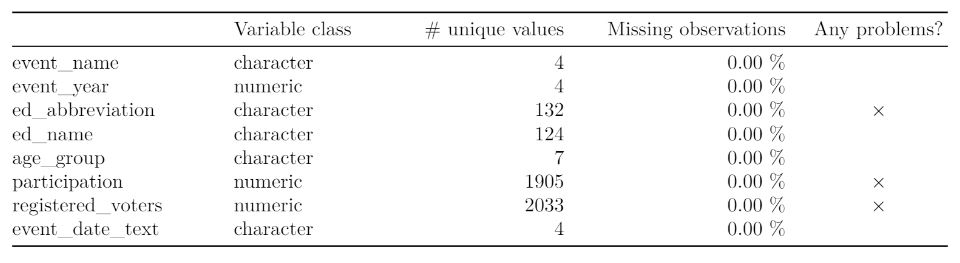
\includegraphics[width=1\linewidth]{../eda/bc_election_turnout_files/figure-html/pvp} \caption{Table 1. Summary of provincial voting participation dataset.}\label{fig:tab_1}
\end{figure}

The pvr dataset contains the number of votes for each candidate and
their respective party broken down again by election and election
district. From this, we can determine how competitive a race was by
calculating the difference in votes between the top two candidates. A
summary of the dataset is shown in Table 2.

\begin{figure}
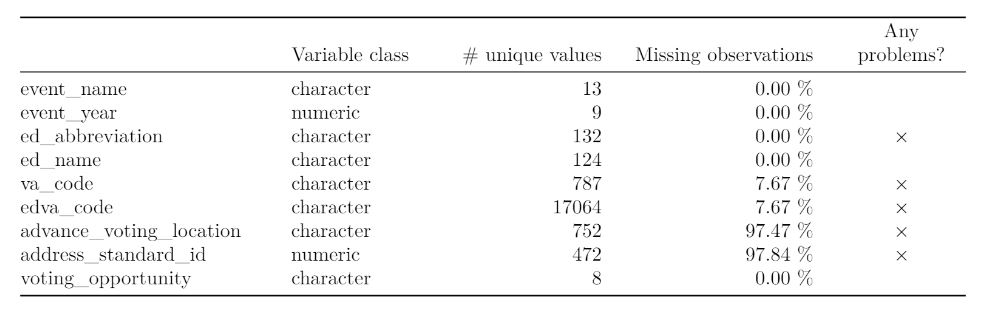
\includegraphics[width=1\linewidth]{../eda/bc_election_turnout_files/figure-html/pvr} \caption{Table 2. Summary of provincial voting results dataset.}\label{fig:unnamed-chunk-1}
\end{figure}

\hypertarget{analysis}{%
\subsection{Analysis}\label{analysis}}

In order to use the \texttt{cor.test()} we need to satisfy ourselves
that the assumptions of \texttt{cor.test()} are sufficiently met. The
first condition of \texttt{cor.test()} is the normality of two
variables. We check the normality using Q-Q plots (quantile-quantile
plots) in Figure 1. These plots show that the normality assumption is
reasonable. The second condition is the linearity of covariation which
can be examined by looking at the scatter plot of two variables (Figure
2). Since a visual inspection of the scatter plot does not seem to
suggest any non-linear pattern, we consider this condition to be valid
as well.

\begin{figure}
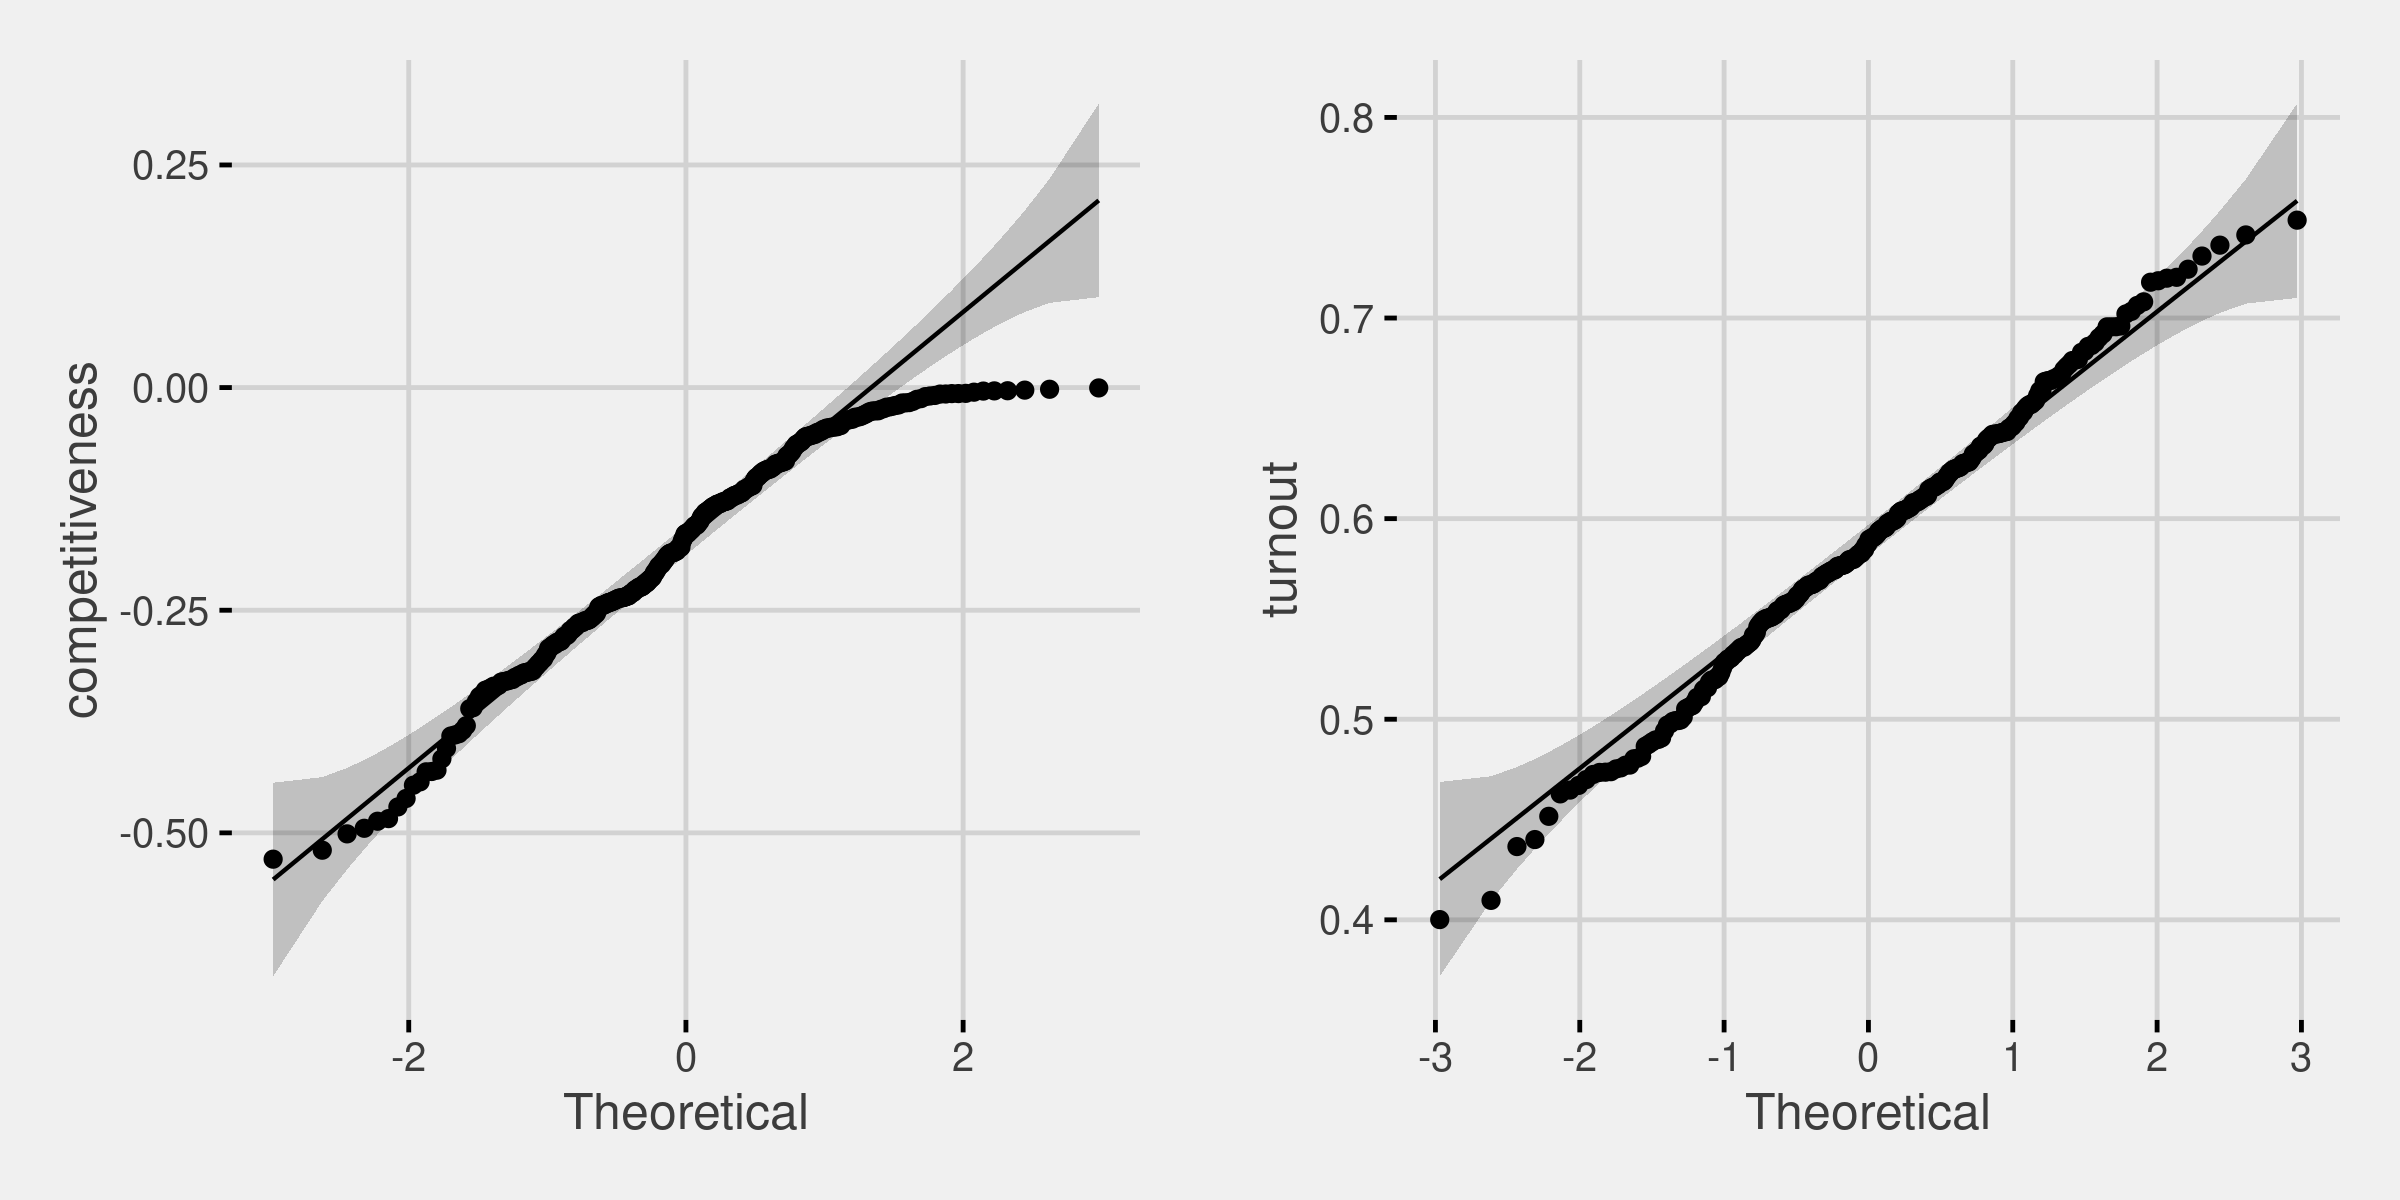
\includegraphics[width=1\linewidth]{images/cow_plot} \caption{Figure 1. Q-Q plot for competitiveness and turnout.}\label{fig:unnamed-chunk-2}
\end{figure}

The scatter plot of competitiveness and turnout is shown in Figure 2. It
shows that an electoral district's competitiveness is potentially
positively correlated with its voter turnout rate. This matches our
expectations. However, in order to understand if their correlation is
statistically significant, we will use a two-sided Pearson correlation
test via \texttt{cor.test()} in R with the following hypotheses:

\begin{quote}
\textbf{Null Hypothesis:} The correlation coefficient between the voter
turnout rate and the race competitiveness is equal to zero.
\end{quote}

\begin{quote}
\textbf{Alternative Hypothesis:} The corrrelation coefficient between
the voter turnout rate and the race competitiveness is not equal to
zero.
\end{quote}

\begin{figure}
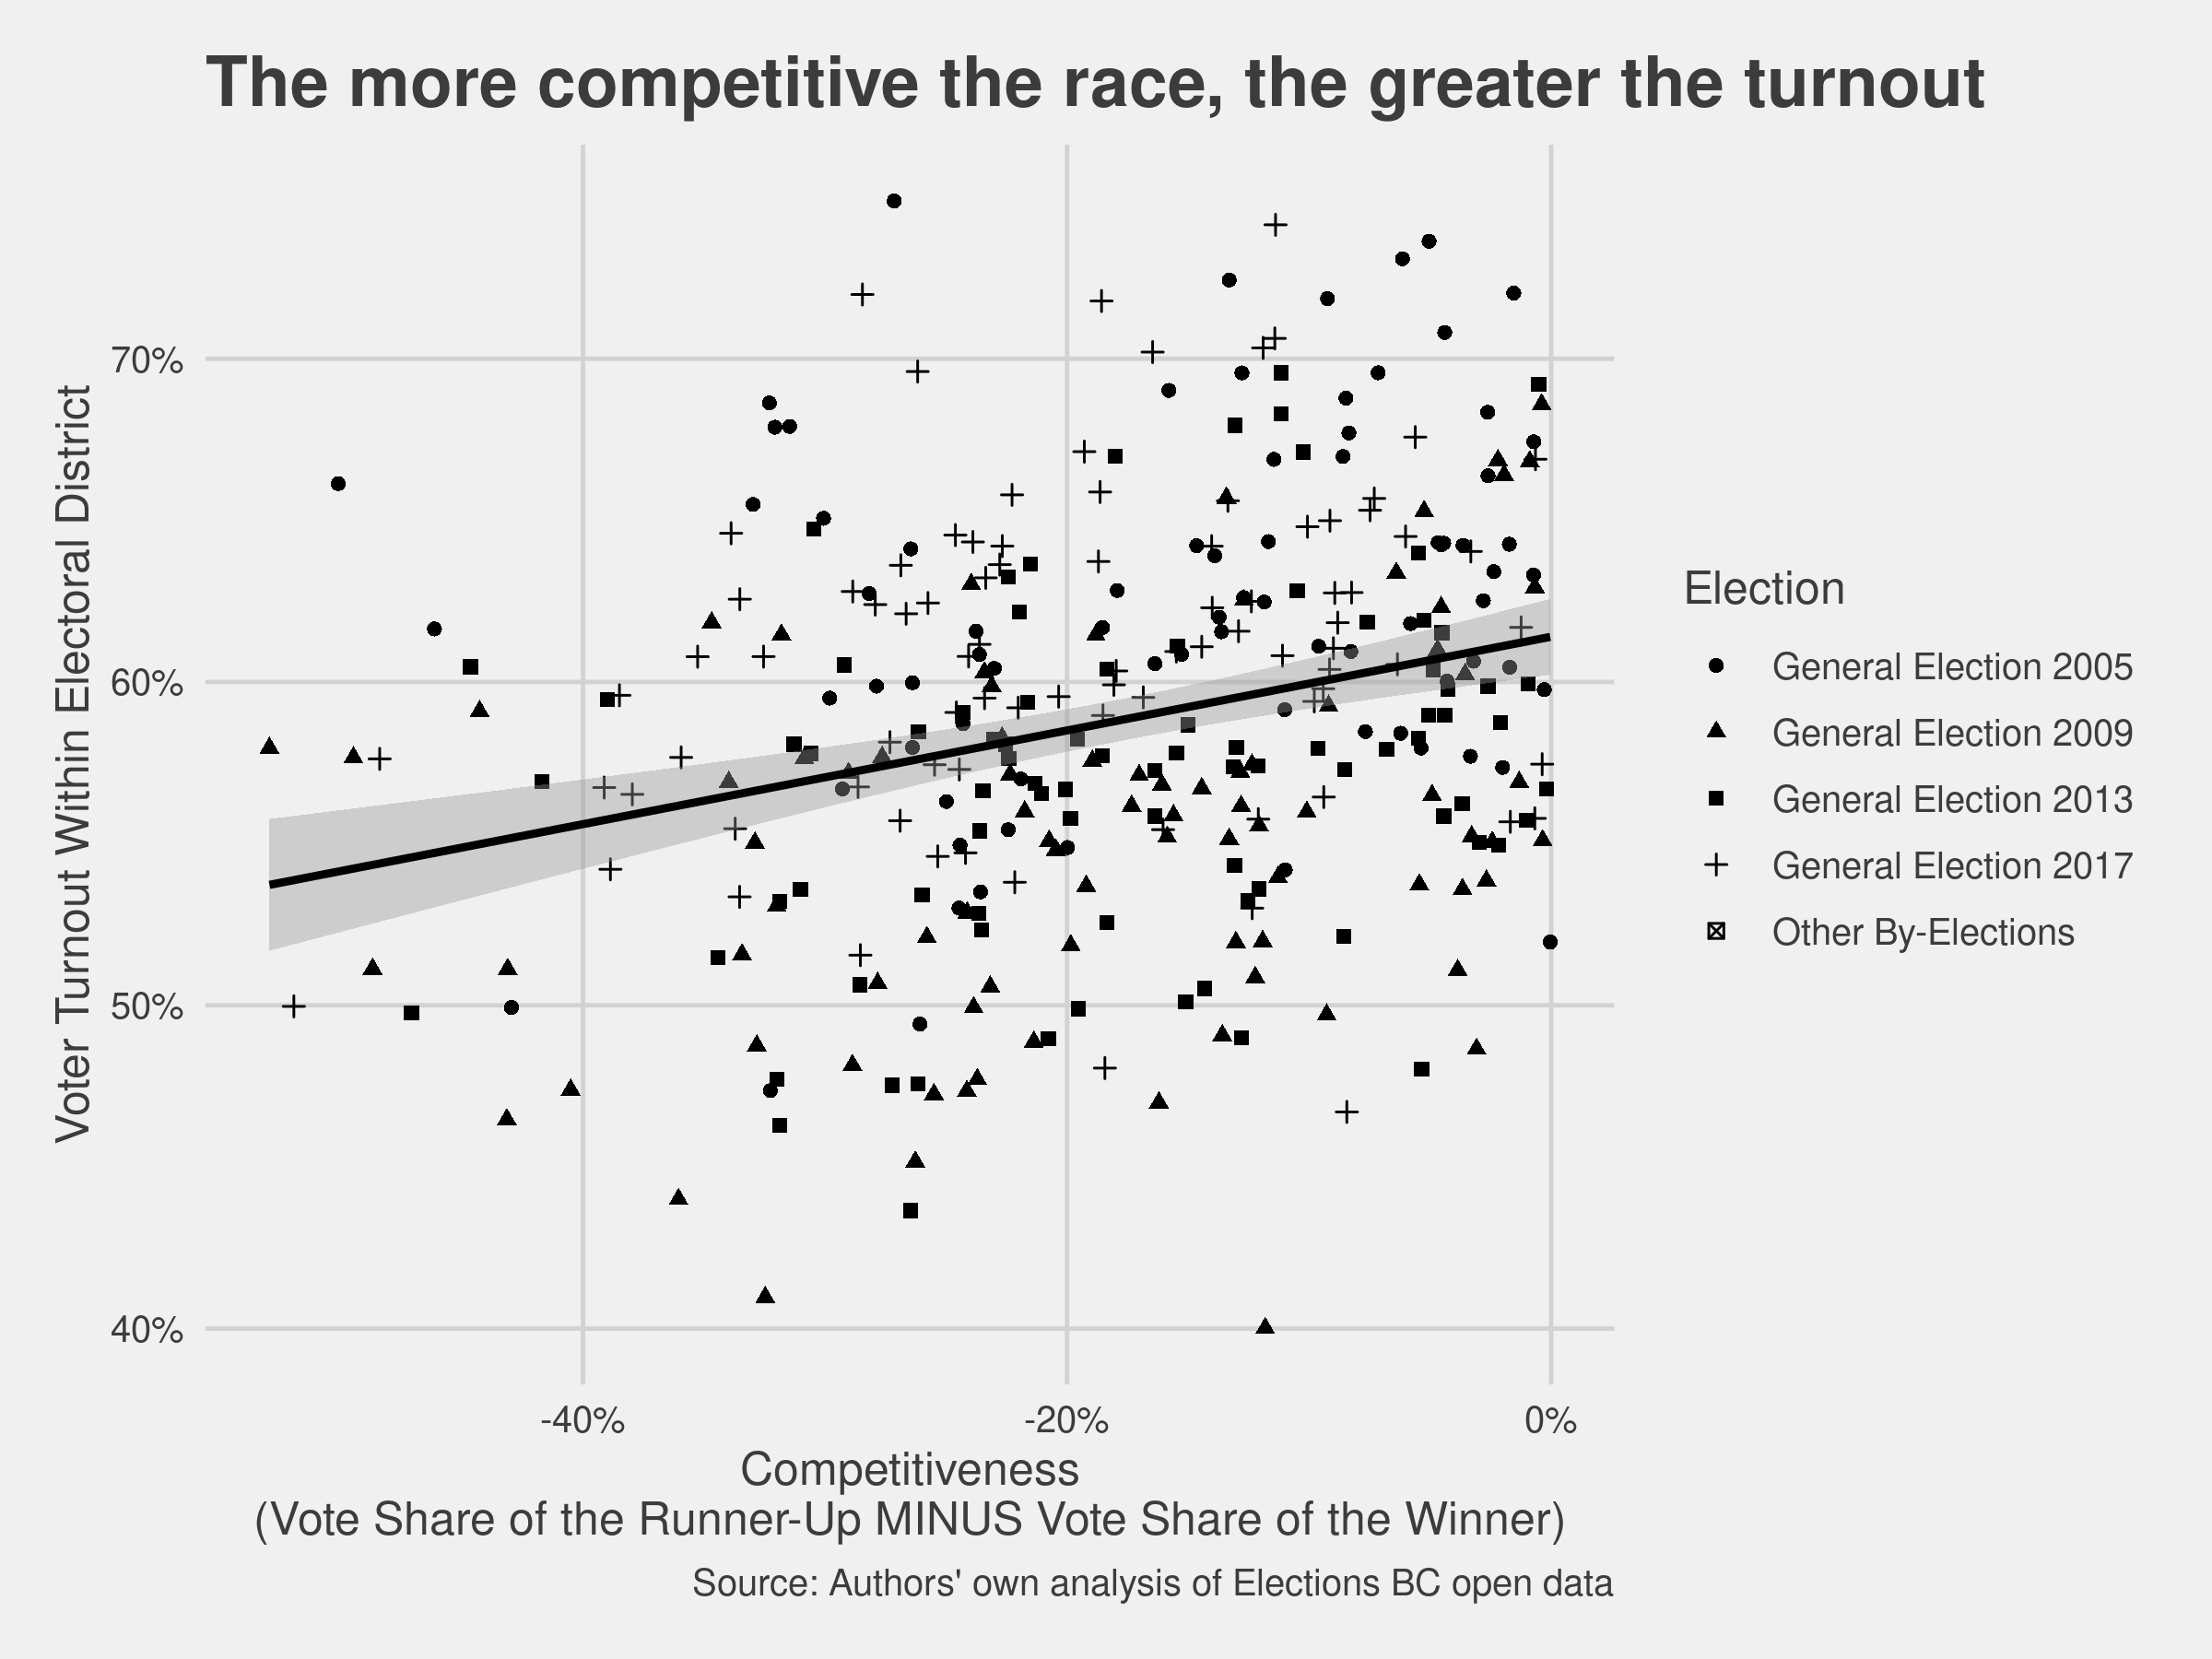
\includegraphics[width=1\linewidth]{images/scatter_plot} \caption{Figure 2. A scatter plot displaying competitiveness vs turnout}\label{fig:unnamed-chunk-3}
\end{figure}

\hypertarget{results-and-discussion}{%
\subsection{Results and Discussion}\label{results-and-discussion}}

Performing the Pearson correlation test in R with \texttt{cor.test()}
produces the results in Table 3. We observe a positive correlation of
0.27 between the competitiveness of a district and its voter turnout.
The final calculated p-value was found to be \(p < .001\). This p-value
falls below our alpha threshold of 0.05, therefore we reject the null
hypothesis and conclude that the linear dependence is statistically
significant.

\begin{longtable}[]{@{}rrrrrrll@{}}
\caption{Table 3. Pearson Correlation Test Results}\tabularnewline
\toprule
\begin{minipage}[b]{0.07\columnwidth}\raggedleft
estimate\strut
\end{minipage} & \begin{minipage}[b]{0.07\columnwidth}\raggedleft
statistic\strut
\end{minipage} & \begin{minipage}[b]{0.06\columnwidth}\raggedleft
p.value\strut
\end{minipage} & \begin{minipage}[b]{0.07\columnwidth}\raggedleft
parameter\strut
\end{minipage} & \begin{minipage}[b]{0.07\columnwidth}\raggedleft
conf.low\strut
\end{minipage} & \begin{minipage}[b]{0.07\columnwidth}\raggedleft
conf.high\strut
\end{minipage} & \begin{minipage}[b]{0.27\columnwidth}\raggedright
method\strut
\end{minipage} & \begin{minipage}[b]{0.09\columnwidth}\raggedright
alternative\strut
\end{minipage}\tabularnewline
\midrule
\endfirsthead
\toprule
\begin{minipage}[b]{0.07\columnwidth}\raggedleft
estimate\strut
\end{minipage} & \begin{minipage}[b]{0.07\columnwidth}\raggedleft
statistic\strut
\end{minipage} & \begin{minipage}[b]{0.06\columnwidth}\raggedleft
p.value\strut
\end{minipage} & \begin{minipage}[b]{0.07\columnwidth}\raggedleft
parameter\strut
\end{minipage} & \begin{minipage}[b]{0.07\columnwidth}\raggedleft
conf.low\strut
\end{minipage} & \begin{minipage}[b]{0.07\columnwidth}\raggedleft
conf.high\strut
\end{minipage} & \begin{minipage}[b]{0.27\columnwidth}\raggedright
method\strut
\end{minipage} & \begin{minipage}[b]{0.09\columnwidth}\raggedright
alternative\strut
\end{minipage}\tabularnewline
\midrule
\endhead
\begin{minipage}[t]{0.07\columnwidth}\raggedleft
0.2727315\strut
\end{minipage} & \begin{minipage}[t]{0.07\columnwidth}\raggedleft
5.18075\strut
\end{minipage} & \begin{minipage}[t]{0.06\columnwidth}\raggedleft
4e-07\strut
\end{minipage} & \begin{minipage}[t]{0.07\columnwidth}\raggedleft
334\strut
\end{minipage} & \begin{minipage}[t]{0.07\columnwidth}\raggedleft
0.1707189\strut
\end{minipage} & \begin{minipage}[t]{0.07\columnwidth}\raggedleft
0.3689592\strut
\end{minipage} & \begin{minipage}[t]{0.27\columnwidth}\raggedright
Pearson's product-moment correlation\strut
\end{minipage} & \begin{minipage}[t]{0.09\columnwidth}\raggedright
two.sided\strut
\end{minipage}\tabularnewline
\bottomrule
\end{longtable}

While the statistical test above does not make any causal claim, the
findings do align with the way many political pundits think about
certain causal relationships in elections. Namely, the common thinking
is that rivaling political parties, informed by pre-election polls,
invest more time and money in campaigning and ``getting out the vote''
in districts they think might swing the election. This behaviour is
likely a product of our ``first-past-the-post'' system, in which the
winner takes all. An interesting angle of analysis to probe this
potential explanation further would be to compare whether this
correlation holds in jurisdictions that use proportional representation.

Subsequent analysis could also continue to build out a model explaining
the voter turnout through multiple regression. Some key variables
explored during the exploratory stages includes marginally predictive
variables such as the election year. Inclusion of additional variables
-- and careful quasi-experimental methods and analysis -- could help
build this model out to a more useful and actionable model for actors in
the political space.

\hypertarget{r-packages}{%
\subsection{R Packages}\label{r-packages}}

This project was carried out using the R programming language (R Core
Team 2020). The following packages were used within R to carry out the
exploratory data analysis and the final analysis: broom (Robinson,
Hayes, and Couch 2020), cowplot (Wilke 2020), dataMaid (Petersen and
Ekstrøm 2019), docopt (de Jonge 2020), dplyr (Wickham, François, et al.
2020), GGally (Schloerke et al. 2020), ggpubr (Kassambara 2020),
ggthemes (Arnold 2019), here (Müller 2020), httr (Wickham 2020a),
janitor (Firke 2020), knitr (Xie 2020), stringr (Wickham 2019), testthat
(Wickham 2011), tidyr (Wickham 2020b), and tidyverse (Wickham, Averick,
et al. 2019).

\hypertarget{references}{%
\subsection*{References}\label{references}}
\addcontentsline{toc}{subsection}{References}

\hypertarget{refs}{}
\leavevmode\hypertarget{ref-ggthemes}{}%
Arnold, Jeffrey B. 2019. \emph{Ggthemes: Extra Themes, Scales and Geoms
for 'Ggplot2'}. \url{https://CRAN.R-project.org/package=ggthemes}.

\leavevmode\hypertarget{ref-docopt}{}%
de Jonge, Edwin. 2020. \emph{Docopt: Command-Line Interface
Specification Language}.
\url{https://CRAN.R-project.org/package=docopt}.

\leavevmode\hypertarget{ref-pvp}{}%
Elections BC. 2018a. 2018.
\url{https://catalogue.data.gov.bc.ca/dataset/6d9db663-8c30-43ec-922b-d541d22e634f/resource/646530d4-078c-4815-8452-c75639962bb4}.

\leavevmode\hypertarget{ref-pvr}{}%
---------. 2018b. 2018.
\url{https://catalogue.data.gov.bc.ca/dataset/44914a35-de9a-4830-ac48-870001ef8935/resource/fb40239e-b718-4a79-b18f-7a62139d9792}.

\leavevmode\hypertarget{ref-BC_elections_license}{}%
``Elections Bc Open Data Licence.'' n.d.
\url{https://www.elections.bc.ca/docs/EBC-Open-Data-Licence.pdf}.

\leavevmode\hypertarget{ref-janitor}{}%
Firke, Sam. 2020. \emph{Janitor: Simple Tools for Examining and Cleaning
Dirty Data}. \url{https://CRAN.R-project.org/package=janitor}.

\leavevmode\hypertarget{ref-ggpubr}{}%
Kassambara, Alboukadel. 2020. \emph{Ggpubr: 'Ggplot2' Based Publication
Ready Plots}. \url{https://CRAN.R-project.org/package=ggpubr}.

\leavevmode\hypertarget{ref-here}{}%
Müller, Kirill. 2020. \emph{Here: A Simpler Way to Find Your Files}.
\url{https://CRAN.R-project.org/package=here}.

\leavevmode\hypertarget{ref-dataMaid}{}%
Petersen, Anne Helby, and Claus Thorn Ekstrøm. 2019. ``dataMaid: Your
Assistant for Documenting Supervised Data Quality Screening in R.''
\emph{Journal of Statistical Software} 90 (6): 1--38.
\url{https://doi.org/10.18637/jss.v090.i06}.

\leavevmode\hypertarget{ref-R}{}%
R Core Team. 2020. \emph{R: A Language and Environment for Statistical
Computing}. Vienna, Austria: R Foundation for Statistical Computing.
\url{https://www.R-project.org/}.

\leavevmode\hypertarget{ref-broom}{}%
Robinson, David, Alex Hayes, and Simon Couch. 2020. \emph{Broom: Convert
Statistical Objects into Tidy Tibbles}.
\url{https://CRAN.R-project.org/package=broom}.

\leavevmode\hypertarget{ref-GGally}{}%
Schloerke, Barret, Di Cook, Joseph Larmarange, Francois Briatte, Moritz
Marbach, Edwin Thoen, Amos Elberg, and Jason Crowley. 2020.
\emph{GGally: Extension to 'Ggplot2'}.
\url{https://CRAN.R-project.org/package=GGally}.

\leavevmode\hypertarget{ref-US_voter_turnout}{}%
``Voter Turnout Is Substantially Higher in Battleground States Than
Spectator States.'' 2020. 2020.
\url{https://www.nationalpopularvote.com/sites/default/files/npv-voter-turnout-memo-v9-2020-5-9.pdf}.

\leavevmode\hypertarget{ref-testthat}{}%
Wickham, Hadley. 2011. ``Testthat: Get Started with Testing.'' \emph{The
R Journal} 3: 5--10.
\url{https://journal.r-project.org/archive/2011-1/RJournal_2011-1_Wickham.pdf}.

\leavevmode\hypertarget{ref-stringr}{}%
---------. 2019. \emph{Stringr: Simple, Consistent Wrappers for Common
String Operations}. \url{https://CRAN.R-project.org/package=stringr}.

\leavevmode\hypertarget{ref-httr}{}%
---------. 2020a. \emph{Httr: Tools for Working with Urls and Http}.
\url{https://CRAN.R-project.org/package=httr}.

\leavevmode\hypertarget{ref-tidyr}{}%
---------. 2020b. \emph{Tidyr: Tidy Messy Data}.
\url{https://CRAN.R-project.org/package=tidyr}.

\leavevmode\hypertarget{ref-tidyverse}{}%
Wickham, Hadley, Mara Averick, Jennifer Bryan, Winston Chang, Lucy
D'Agostino McGowan, Romain François, Garrett Grolemund, et al. 2019.
``Welcome to the tidyverse.'' \emph{Journal of Open Source Software} 4
(43): 1686. \url{https://doi.org/10.21105/joss.01686}.

\leavevmode\hypertarget{ref-dplyr}{}%
Wickham, Hadley, Romain François, Lionel Henry, and Kirill Müller. 2020.
\emph{Dplyr: A Grammar of Data Manipulation}.
\url{https://CRAN.R-project.org/package=dplyr}.

\leavevmode\hypertarget{ref-cowplot}{}%
Wilke, Claus O. 2020. \emph{Cowplot: Streamlined Plot Theme and Plot
Annotations for 'Ggplot2'}.
\url{https://CRAN.R-project.org/package=cowplot}.

\leavevmode\hypertarget{ref-knitr}{}%
Xie, Yihui. 2020. \emph{Knitr: A General-Purpose Package for Dynamic
Report Generation in R}. \url{https://yihui.org/knitr/}.

\end{document}
